\documentclass[UTF8,fontset=fandol,11pt,a4paper]{ctexart}
\usepackage[margin=22mm]{geometry}
\usepackage{amsmath,amssymb,booktabs,graphicx,float,array,enumitem,xcolor,hyperref}
\hypersetup{colorlinks=true,linkcolor=blue!50!black,urlcolor=blue!50!black,
  pdftitle={Q1：二维格点上的三玻色子模型}}
\setlist{itemsep=2pt,topsep=3pt,leftmargin=1.8em}
\setlength{\parskip}{4pt}
\linespread{1.15}
\ctexset{section={format=\Large\bfseries,beforeskip=14pt,afterskip=6pt},
         subsection={format=\large\bfseries,beforeskip=10pt,afterskip=4pt}}
\newenvironment{keybox}[1]
  {\par\noindent\setlength{\fboxsep}{8pt}\setlength{\fboxrule}{0.6pt}%
   \begin{lrbox}{0}\begin{minipage}{\dimexpr\linewidth-2\fboxsep-2\fboxrule\relax}%
   {\bfseries\color{blue!45!black}#1}\par\smallskip}
  {\end{minipage}\end{lrbox}\fcolorbox{blue!45!black}{blue!3}{\usebox{0}}\par}
\newcommand{\Etwo}{-0.820776322}
\newcommand{\Eground}{-4.771434366}
\newcommand{\Eexcited}{-1.108993749}
\newcommand{\Erel}{-0.288217427}
\newcommand{\Binding}{3.950658045}
\newcommand{\CstarMax}{4.2910935}
\newcommand{\Lmax}{40}
\newcommand{\LastRootChange}{0.000982}
\newcommand{\RmsGround}{0.673}
\newcommand{\RmsExcited}{2.144}
\newcommand{\MaxResidual}{7.31\times10^{-11}}
\newcommand{\MaxSymmetry}{1.13\times10^{-10}}
\newcommand{\MaxOrtho}{1.49\times10^{-14}}
\newcommand{\Nsolves}{152}

\newcommand{\rr}{\mathbf r}
\newcommand{\dd}{\boldsymbol\delta}
\newcommand{\Ethr}{E_{\mathrm{thr}}}

\begin{document}

\begin{center}
{\LARGE\bfseries Q1：从 $^8$Be 到玩具碳核}\\[6pt]
{\large 二维周期格点上三玻色子模型的推导、求解与验证}\\[4pt]
{\small TIF345/FYM345 \quad Project: \textit{Fine-tuned for life?}}
\end{center}

\begin{keybox}{题目（Q1 原文）}
\textit{Compute the threshold and the $0^+_1$ and $0^+_2$ states (a sparse eigensolver in the full space suffices),
and verify their symmetry. How do they and the threshold depend on $c\in[3.5,7]$ and $L$, and at which $c^\star$
does the Hoyle-like state cross the threshold? How do you know that your results are right?}

\medskip
\textbf{结论速览。}
(1) $c=5,L=20$ 时 $\Ethr=-0.821$，$E_{3,1}=-4.771$，$E_{3,2}=-1.109$，复现题目基准；
(2) 所有能级随 $c$ 单调下降，Hoyle-like 态下降快于阈值，因此由阈值上方穿到下方；
(3) 穿越点依赖盒子大小，大盒子收敛到 $c^\star\approx4.29$；
(4) 解析极限、对称性、导数与收敛检查共同保证结果正确。
\end{keybox}

%====================================================================
\section{理论推导}

\subsection{模型}
三个质量为 $m$ 的相同玻色子位于 $L\times L$ 周期格点（格距 $a$）：
\begin{equation}
H=-\frac{\hbar^2}{2m}\sum_{i=1}^{3}\nabla_i^2+\sum_{i<j}V_c(|\mathbf x_i-\mathbf x_j|),\qquad
V_c(r)=-c\,\underbrace{e^{-r^2}}_{f(r)}+\underbrace{\frac{0.3}{\sqrt{r^2+1}}}_{g(r)}.
\end{equation}
$f$ 是强度为 $c$ 的短程吸引（“强力”），$g$ 是弱的长程排斥（“库仑”）。记 $t=\hbar^2/(2ma^2)$，数值上取 $a=t=1$。
周期盒子中的距离取最小镜像 $d_L(\rr)=\min_{\mathbf n\in\mathbb Z^2}|\rr+La\,\mathbf n|$。

\subsection{第一步：把动能放到格点上}
Taylor 展开 $\phi(x\pm a)$ 并相加，奇数阶项相消：
\begin{equation}
-\frac{\hbar^2}{2m}\phi''(x)=t\,[2\phi(x)-\phi(x+a)-\phi(x-a)]+O(a^2).
\end{equation}
用周期移位矩阵 $(S\phi)_n=\phi_{(n+1)\bmod L}$，一维动能为 $t(2I-S-S^T)$；二维令 $S_x=S\otimes I$、$S_y=I\otimes S$：
\begin{equation}
(T_1\phi)(\mathbf x)=4t\,\phi(\mathbf x)-t\sum_{\dd}\phi(\mathbf x+\dd),\qquad \dd\in\{\pm\hat x,\pm\hat y\}.
\end{equation}
\textbf{记住一条规则：}每个粒子贡献对角元 $4t$，它的每一种最近邻跳跃贡献 $-t$；势能在位置基底中是对角的。

\subsection{第二步：平移不变性 $\Rightarrow$ 相对坐标}
整体平移 $\mathbf x_i\mapsto\mathbf x_i+\mathbf b$ 不改变跳跃，也不改变粒子间距，因此与 $H$ 对易，总动量 $\mathbf K$ 守恒。
我们只需质心静止的 $\mathbf K=0$ 分块，其中波函数只依赖相对坐标。这把维数从 $L^{2n}$ 降到 $L^{2(n-1)}$。

\paragraph{两体。}令 $\rr=\mathbf x_1-\mathbf x_2$，$\Psi(\mathbf x_1,\mathbf x_2)=\phi(\rr)$。
粒子 1 跳 $\dd$ 给出 $\phi(\rr+\dd)$，粒子 2 跳 $\dd$ 给出 $\phi(\rr-\dd)$；由于 $\{\dd\}$ 关于原点对称，两项相等：
\begin{equation}
\boxed{(H_2\phi)(\rr)=8t\,\phi(\rr)-2t\sum_{\dd}\phi(\rr+\dd)+V_c\big(d_L(\rr)\big)\,\phi(\rr)}
\label{eq:h2}
\end{equation}
跳跃系数 $2t$ 对应约化质量 $\mu=m/2$。矩阵维数 $L^2$。

\paragraph{阈值。}“两体束缚态 + 一个相对静止的粒子”的能量就是两体基态能量加零：
\begin{equation}
\Ethr=E_2=\min\operatorname{spec}(H_2),\qquad
E_R=E_{3,2}-\Ethr,\qquad B=\Ethr-E_{3,1},\qquad E_R(c^\star)=0.
\end{equation}

\paragraph{三体。}令 $\rr_1=\mathbf x_1-\mathbf x_3$、$\rr_2=\mathbf x_2-\mathbf x_3$。每个粒子跳一次的效果：
\begin{center}
\begin{tabular}{lll}
\toprule
粒子跳跃 & $(\rr_1,\rr_2)$ 变为 & \\
\midrule
$\mathbf x_1\to\mathbf x_1+\dd$ & $(\rr_1+\dd,\ \rr_2)$ & 只动 $\rr_1$ \\
$\mathbf x_2\to\mathbf x_2+\dd$ & $(\rr_1,\ \rr_2+\dd)$ & 只动 $\rr_2$ \\
$\mathbf x_3\to\mathbf x_3+\dd$ & $(\rr_1-\dd,\ \rr_2-\dd)$ & \textbf{两者同时动} \\
\bottomrule
\end{tabular}
\end{center}
对角动能 $3\times4t=12t$，跳跃共 $3\times4=12$ 个：
\begin{equation}
\boxed{\begin{aligned}
(H_3\psi)(\rr_1,\rr_2)={}&12t\,\psi-t\sum_{\dd}\Big[\psi(\rr_1{+}\dd,\rr_2)+\psi(\rr_1,\rr_2{+}\dd)+\psi(\rr_1{-}\dd,\rr_2{-}\dd)\Big]\\
&+\Big[V_c\big(d_L(\rr_1)\big)+V_c\big(d_L(\rr_2)\big)+V_c\big(d_L(\rr_1-\rr_2)\big)\Big]\psi
\end{aligned}}
\label{eq:h3}
\end{equation}
斜向项来自粒子 3，是连续动能 $-\tfrac{\hbar^2}{m}(\nabla_1^2+\nabla_2^2+\nabla_1\!\cdot\!\nabla_2)$ 中交叉项的格点对应。

\begin{figure}[H]
\centering
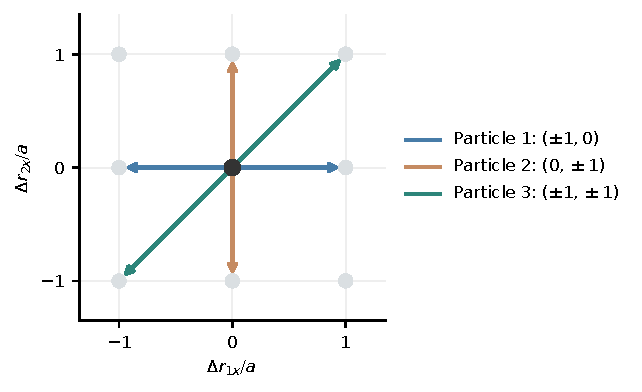
\includegraphics[width=.62\textwidth]{../figures/relative_hops.pdf}
\caption{相对坐标中的跳跃方向（$x$ 分量；$y$ 同理）。绿色斜向跳跃来自粒子 3。}
\end{figure}

\paragraph{矩阵形式。}全部问题写成
\begin{equation}
H(c)=T+G-c\,F,
\end{equation}
$T$ 为稀疏动能，$F,G$ 为对角势能（对所有粒子对求和）。$H$ 是\textbf{实对称}矩阵，三体维数 $L^4$ 但每行只有 13 个非零元；
$T,F,G$ 与 $c$ 无关，改变 $c$ 只改对角线。

\subsection{第三步：对称性与 $0^+$ 的定义}
$H$ 有两类对称操作，都是构型之间的置换：
\begin{itemize}
\item \textbf{玻色交换 $S_3$}，生成元 $P_{12}:(\rr_1,\rr_2)\mapsto(\rr_2,\rr_1)$，
      $P_{13}:(\rr_1,\rr_2)\mapsto(-\rr_1,\ \rr_2-\rr_1)$（由 $\mathbf x_1\leftrightarrow\mathbf x_3$ 直接代入得到）。
\item \textbf{格点点群 $D_4$}，生成元 $R_{90}:(x,y)\mapsto(-y,x)$，$M_x:(x,y)\mapsto(x,-y)$，同时作用于 $\rr_1,\rr_2$。
\end{itemize}
它们把跳跃映为跳跃、把粒子对映为粒子对，并保持 $d_L$，因此 $[H,\mathcal S]=0$。
正方格点没有连续转动，“$0^+$”的格点对应是：$S_3$ 全对称且属于 $D_4$ 的平凡表示 $A_1$。在生成元下不变即在整个群下不变：
\begin{equation}
\psi\in0^+\iff \mathcal S\psi=\psi,\qquad \mathcal S\in\{P_{12},P_{13},R_{90},M_x\}.
\end{equation}
对归一化实本征向量，若属于其他一维表示则某个 $\|\mathcal S\psi-\psi\|=2$，二维表示也给出 $O(1)$ 的值；对称态与非对称态之间有清楚的数量级差距。

\subsection{第四步：能级如何随 $c$ 变化}
对非简并归一化本征态，Hellmann--Feynman 定理给出
\begin{equation}
\frac{\partial E_n}{\partial c}=\Big\langle\frac{\partial H}{\partial c}\Big\rangle_n=-\langle F\rangle_n\le0 .
\end{equation}
因为 $F\ge0$，\textbf{增大吸引使所有能级下降}。但
$\dfrac{dE_R}{dc}=-\langle F_3\rangle_{0^+_2}+\langle F_2\rangle_{2}$ 的符号取决于两个期望值的大小，必须由计算决定——这就是穿越问题的实质。
$H(c)$ 对 $c$ 是线性的，非简并本征值连续可微，若 $E_R$ 在区间两端变号，介值定理保证区间内有根 $c^\star$。

\subsection{第五步：两个可解析的检验}\label{sec:analytic}
\paragraph{自由谱。}令 $V=0$，代入平面波 $\psi=e^{i(\mathbf k\cdot\rr_1+\mathbf q\cdot\rr_2)}$，由式~\eqref{eq:h3}：
\begin{equation}
T_3\psi=\big[\epsilon(\mathbf k)+\epsilon(\mathbf q)+\epsilon(\mathbf k+\mathbf q)\big]\psi,\qquad
\epsilon(\mathbf k)=2t\sum_{\mu}[1-\cos(k_\mu a)],
\end{equation}
恰为三粒子动量 $\mathbf k,\mathbf q,-(\mathbf k+\mathbf q)$ 的自由能量；两体同理为 $2\epsilon(\mathbf k)$。
漏掉斜向项或把两体系数写成 $t$，都会破坏这一等式，因此它直接检验了推导。

\paragraph{有限体积。}束缚态在远处 $\psi\sim e^{-\kappa r}$，$\kappa\propto\sqrt{|E_{\rm bind}|}$。周期盒子使波函数与镜像重叠，修正约为
$\Delta E(L)\sim e^{-\kappa La}$：\textbf{态越松散，收敛越慢}。在 $c^\star$ 附近 Hoyle-like 态最贴近阈值、也最松散，所以 $c^\star(L)$ 是最难收敛的量。

%====================================================================
\section{数值方法}

\subsection{Lanczos：只求最低几个态}
$L^4\times L^4$ 稠密对角化不可行，但只需最低少数几个态，而稀疏矩阵乘向量仅 $O(L^4)$。
Lanczos 在 Krylov 子空间 $\mathcal K_m=\mathrm{span}\{q,Hq,\dots,H^{m-1}q\}$ 中用三项递推构造正交基：
\begin{equation}
w=Hq_j-\beta_{j-1}q_{j-1},\quad \alpha_j=q_j^Tw,\quad w\leftarrow w-\alpha_jq_j,\quad \beta_j=\|w\|,\quad q_{j+1}=w/\beta_j,
\end{equation}
把 $H$ 投影成三对角矩阵 $T_m$（对角 $\alpha_j$，次对角 $\beta_j$）。对角化 $T_m$ 得 Ritz 值 $\theta$ 与 Ritz 向量 $y$；谱两端收敛最快。
实际使用 SciPy \texttt{eigsh(which='SA')}（ARPACK 隐式重启 Lanczos）。

\textbf{收敛判据。}对实对称矩阵，若 $\rho=\|Hy-\theta y\|$，则必有本征值 $\lambda$ 满足 $|\lambda-\theta|\le\rho$。
我们在原空间重新计算 $\rho$，不只依赖求解器的停止标志。

\subsection{选态与求根}
\begin{enumerate}
\item 求 $H_2$ 最低态得 $\Ethr$。
\item 在\emph{完整}空间求 $H_3$ 最低 $k$ 个态，按能量升序排列。
\item 对每个态检验四个生成元的 $\|\mathcal S\psi-\psi\|$；取前两个通过者为 $0^+_1,0^+_2$。不足两个则 $k\to2k$ 重算。
\item 在 $c\in[3.5,7]$ 上扫描 $E_R(c)$，对变号区间用 Brent 法求 $c^\star$。
\item 依次增大 $L$，比较 $E(L)$ 和 $c^\star(L)$ 的相邻差，作为收敛判据。
\end{enumerate}
不预先投影到对称子空间：既避免投影实现出错，又能确认没有更低的对称态被遗漏。

%====================================================================
\section{验证：怎么知道结果是对的}
\begin{table}[H]
\centering
\begin{tabular}{p{0.40\textwidth}p{0.22\textwidth}p{0.26\textwidth}}
\toprule
检查 & 检验对象 & 最大误差 \\
\midrule
自由谱 vs.\ 解析色散（$L=3$ 全谱） & 推导与系数 & $2.3\times10^{-14}$ \\
$H=H^T$；常数态 $T\mathbf 1=0$ & 矩阵组装 & 精确为 0 \\
$[H,\mathcal S]$ 作用于随机向量 & 对称操作 & $1.3\times10^{-16}$ \\
稠密 vs.\ 稀疏（$L=3$） & 本征求解器 & $2.7\times10^{-15}$ \\
Hellmann--Feynman vs.\ 数值差分 & 本征向量 & $2.4\times10^{-10}$ \\
换随机种子、容差 $10^{-12}$ & 伪收敛 & $1.5\times10^{-14}$ \\
\midrule
全部 \Nsolves\ 个求解点：残差 $\rho$ & 每个结果 & $\MaxResidual$ \\
全部求解点：目标态对称误差 & 选态 & $\MaxSymmetry$ \\
题目基准（$c=5,L=20$） & 模型约定 & 三位小数一致 \\
增大 $L$ 至 \Lmax & 有限体积 & 见第~\ref{sec:fv} 节 \\
\bottomrule
\end{tabular}
\end{table}
\noindent 前几项保证“在给定 $L$ 下算得对”，最后一项单独回答“盒子够不够大”。

%====================================================================
\section{结果}

\subsection{基准点与 $c$ 依赖}
$c=5$、$L=20$：
$\Ethr=\Etwo$，$E_{3,1}=\Eground$，$E_{3,2}=\Eexcited$，
$E_R=\Erel$，$B=\Binding$。
在全部采样点，选出的两个 $0^+$ 态恰为整个谱中最低的两个态。

\begin{figure}[H]
\centering
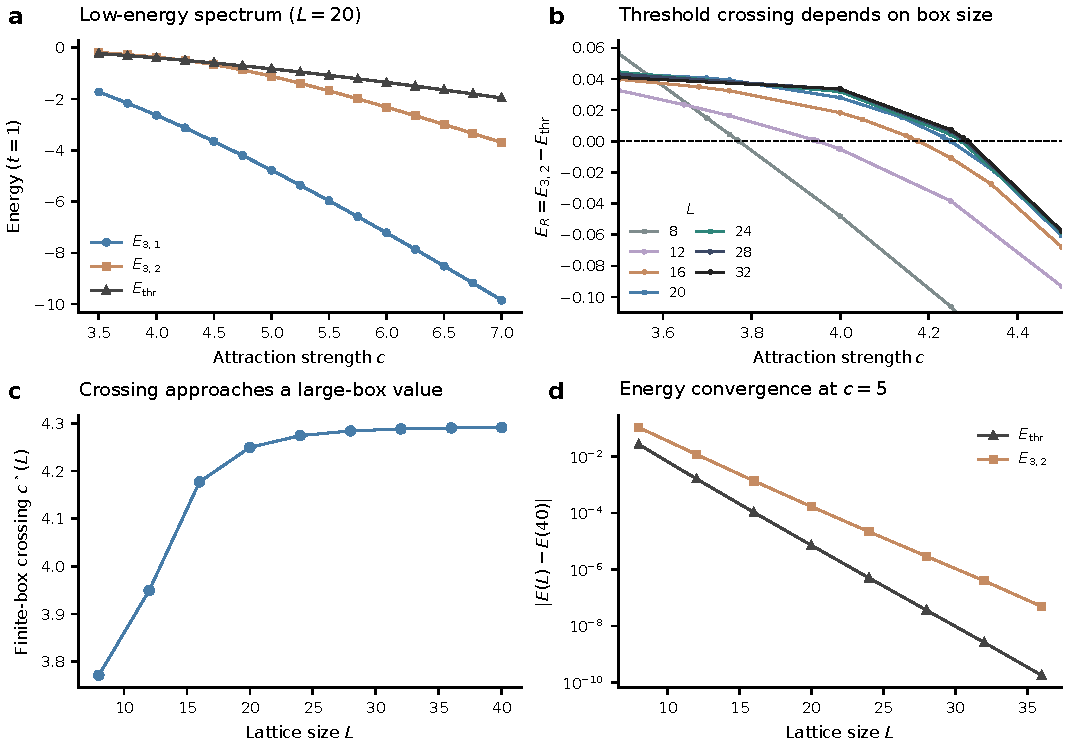
\includegraphics[width=\textwidth]{../figures/spectrum_convergence.pdf}
\caption{\textbf{a} $L=20$ 能级随 $c$ 单调下降。\textbf{b} $E_R(c)$ 自上而下穿过零，穿越点随 $L$ 右移。
\textbf{c} $c^\star(L)$ 趋于平台。\textbf{d} $c=5$ 能量与 $L=40$ 之差，按指数减小。}
\label{fig:spectrum}
\end{figure}

\subsection{有限体积与穿越点}\label{sec:fv}
\begin{table}[H]
\centering\small
\begin{tabular}{rrrrr}\toprule $L$ & $E_2$ ($c=5$) & $E_{3,1}$ ($c=5$) & $E_{3,2}$ ($c=5$) & $c^\star(L)$ \\ \midrule
8 & -0.847376048 & -4.771681772 & -1.214088937 & 3.7717075 \\
12 & -0.822388617 & -4.771434751 & -1.120646222 & 3.9493804 \\
16 & -0.820874284 & -4.771434367 & -1.110186317 & 4.1770508 \\
20 & -0.820776322 & -4.771434366 & -1.108993749 & 4.2494228 \\
24 & -0.820769644 & -4.771434366 & -1.108848047 & 4.2741346 \\
28 & -0.820769174 & -4.771434366 & -1.108829219 & 4.2838791 \\
32 & -0.820769140 & -4.771434366 & -1.108826687 & 4.2881251 \\
36 & -0.820769138 & -4.771434366 & -1.108826337 & 4.2901120 \\
40 & -0.820769138 & -4.771434366 & -1.108826287 & 4.2910935 \\
\bottomrule\end{tabular}

\caption{$c=5$ 的能量与各 $L$ 的穿越点。}
\end{table}
\begin{itemize}
\item 基态紧凑，$L\ge20$ 时 9 位小数不变；阈值与 Hoyle-like 态收敛较慢；$c^\star(L)$ 最慢。
\item $c^\star$ 从 3.77（$L=8$）升到 \CstarMax（$L=\Lmax$），最后一步仅变化 \LastRootChange，远大于求根容差 $2\times10^{-7}$。
      因此精度由有限体积决定：$\boxed{c^\star\approx4.29}$。
\item $L=20$ 足以复现基准，但会把穿越点低估为 4.249。
\end{itemize}

\subsection{空间结构：为什么 Hoyle-like 态更敏感}
粒子对分布 $P(\rr_1)=\sum_{\rr_2}|\psi|^2$，均方根间距 $r_{\rm rms}=[\sum d_L(\rr_1)^2P(\rr_1)]^{1/2}$：
基态 $\RmsGround\,a$，Hoyle-like 态 $\RmsExcited\,a$，约大 3 倍，与第~\ref{sec:analytic} 节的有限体积论证一致。
\begin{figure}[H]
\centering
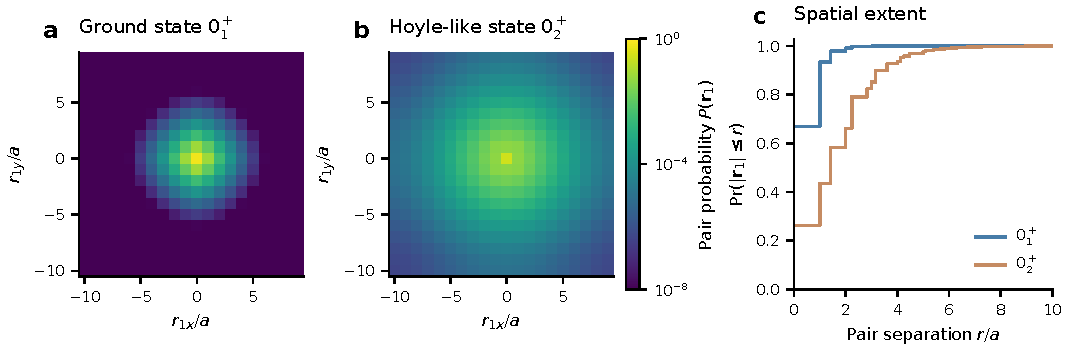
\includegraphics[width=\textwidth]{../figures/state_structure.pdf}
\caption{$c=5,L=20$。\textbf{a,b} 两个态的粒子对分布（同一对数色标）。\textbf{c} 间距的累积概率。}
\end{figure}

%====================================================================
\section{结论}
\begin{enumerate}
\item 由单粒子跳跃规则和平移不变性导出两体（系数 $2t$）与三体（含粒子 3 的斜向跳跃）相对坐标哈密顿量。
\item 在完整空间用 Lanczos 求最低态，按 $S_3\times D_4$ 生成元筛出 $0^+_1,0^+_2$，复现题目基准。
\item 所有能级随 $c$ 下降；Hoyle-like 态下降更快，于 $c^\star\approx4.29$ 穿过阈值。该值需要 $L\gtrsim28$ 才稳定到 $10^{-2}$ 以内。
\item 解析自由谱、对称对易、Hellmann--Feynman、残差界与 $L$ 收敛分别检验了推导、实现和物理盒子大小。
\end{enumerate}
\textbf{适用范围：}固定格距 $a=1$ 的格点模型，未做连续极限；有限盒子中的离散能级不等同于无限体积共振。

\end{document}
